% Shared results; numeric tables are generated directly from completed summaries.
\section{Results and Discussion of the Replicated Study}
\label{sec:results}

\subsection{Higher Excess Entropy Selected by HNC}

Table~\ref{tab:new_states} reports the new dense-state results; these replace the earlier single-trajectory transport estimates as the evidence for component-dependent mobility. The corresponding absolute-state intervals are given in Table~\ref{tab:new_intervals}. HNC successfully selects higher-excess-entropy liquids: H5 relative to U4 has $\Delta s_{\rm ex}=+0.1107k_B$ in HNC and $+0.10322k_B$ in MD. With monovalent background, H7 relative to U6 gives $+0.1108k_B$ and $+0.10331k_B$, respectively. Absolute HNC entropies remain more negative than MD by approximately $0.064$--$0.093k_B$ per particle. Agreement of increments is better than agreement of absolute values.

% Generated by generate_component_study_assets.py; do not edit numbers by hand.
\begin{table*}[t]
\centering
\caption{Dense-state HNC excess entropy and replicated MD means at $T^*=2$, $\rho^*=0.7$, $N=4000$. Diffusion coefficients are in $\sigma^2/\tau$; $D_{\rm probe}=(D_{+2}+D_{-2})/2$. MD uses the primary 20--100$\tau$ MSD fitting window. L5 is an exact mechanical duplicate of U4 and is excluded from entropy-scaling fits. Confidence intervals for the primary comparisons are reported in Table~\ref{tab:new_contrasts}; absolute-state intervals are in Table~\ref{tab:new_intervals}.}
\label{tab:new_states}
\small
\resizebox{\ifdim\width>\textwidth\textwidth\else\width\fi}{!}{%
\begin{tabular}{lrrrrrr}
\toprule
State & HNC $s_{\rm ex}/k_B$ & MD $s_{\rm ex}/k_B$ & $D_{\rm net}$ & $D_{\rm probe}$ & $D_{+2}$ & $D_{-2}$ \\
\midrule
B3 & -2.06350 & -1.97101 & 0.22253 & 0.20677 & 0.21196 & 0.20158 \\
B5 & -2.06770 & -1.97421 & 0.22279 & 0.21047 & 0.20879 & 0.21214 \\
U4 & -1.84340 & -1.77209 & 0.25945 & 0.23684 & 0.23913 & 0.23455 \\
L5 & -1.84340 & -1.77166 & 0.25945 & 0.23684 & 0.23913 & 0.23455 \\
M5 & -1.81020 & -1.74170 & 0.26720 & 0.24038 & 0.23937 & 0.24139 \\
H5 & -1.73270 & -1.66887 & 0.28401 & 0.24825 & 0.24764 & 0.24885 \\
U6 & -1.84780 & -1.77603 & 0.26018 & 0.23572 & 0.23742 & 0.23401 \\
H7 & -1.73700 & -1.67272 & 0.28196 & 0.24795 & 0.24634 & 0.24956 \\
\bottomrule
\end{tabular}}
\end{table*}

% Generated by generate_component_study_assets.py; do not edit numbers by hand.
\begin{table*}[t]
\centering
\caption{Absolute-state nominal 95\% Student-$t$ intervals across three independent replicas. Because the states are paired by replica, interval overlap here is not a test of the paired differences in Table~\ref{tab:new_contrasts}. These intervals exclude systematic uncertainty.}
\label{tab:new_intervals}
\small
\resizebox{\ifdim\width>\textwidth\textwidth\else\width\fi}{!}{%
\begin{tabular}{lrrr}
\toprule
State & $s_{\rm ex}/k_B$ & $D_{\rm net}$ & $D_{\rm probe}$ \\
\midrule
B3 & $[-1.97339,-1.96864]$ & $[0.21959,0.22546]$ & $[0.20364,0.20991]$ \\
B5 & $[-1.97657,-1.97186]$ & $[0.22095,0.22463]$ & $[0.20626,0.21468]$ \\
U4 & $[-1.77342,-1.77076]$ & $[0.25884,0.26005]$ & $[0.23336,0.24032]$ \\
L5 & $[-1.77421,-1.76912]$ & $[0.25884,0.26005]$ & $[0.23336,0.24032]$ \\
M5 & $[-1.74422,-1.73917]$ & $[0.26358,0.27082]$ & $[0.22969,0.25107]$ \\
H5 & $[-1.66936,-1.66838]$ & $[0.28214,0.28588]$ & $[0.23921,0.25728]$ \\
U6 & $[-1.77667,-1.77539]$ & $[0.25480,0.26557]$ & $[0.21782,0.25361]$ \\
H7 & $[-1.67584,-1.66960]$ & $[0.27882,0.28511]$ & $[0.23406,0.26183]$ \\
\bottomrule
\end{tabular}}
\end{table*}

% Generated by generate_component_study_assets.py; do not edit numbers by hand.
\begin{table*}[t]
\centering
\caption{Paired composition changes, numerator relative to denominator. Brackets are nominal 95\% Student-$t$ intervals from three independent replica pairs (two degrees of freedom), without multiple-comparison correction. Diffusion changes are $100[\exp(\overline{\ln(D_a/D_b)})-1]$ and intervals are transformed in the same way. Entropy differences are per particle in $k_B$. Intervals quantify replica sampling, excluding estimator and finite-size bias.}
\label{tab:new_contrasts}
\small
\resizebox{\ifdim\width>\textwidth\textwidth\else\width\fi}{!}{%
\begin{tabular}{lrrr}
\toprule
Comparison & $\Delta s_{\rm ex}/k_B$ [95\% CI] & $\Delta D_{\rm net}$ (\%) [95\% CI] & $\Delta D_{\rm probe}$ (\%) [95\% CI] \\
\midrule
L5/U4 & $+0.00042\;[-0.00219,+0.00304]$ & $+0.00\;[+0.00,+0.00]$ & $+0.00\;[+0.00,+0.00]$ \\
M5/U4 & $+0.03039\;[+0.02727,+0.03352]$ & $+2.99\;[+1.38,+4.62]$ & $+1.48\;[-1.57,+4.64]$ \\
H5/U4 & $+0.10322\;[+0.10209,+0.10434]$ & $+9.47\;[+8.96,+9.97]$ & $+4.81\;[+0.60,+9.19]$ \\
H5/B3 & $+0.30214\;[+0.29927,+0.30501]$ & $+27.63\;[+25.40,+29.90]$ & $+20.05\;[+14.30,+26.09]$ \\
H7/U6 & $+0.10331\;[+0.09990,+0.10672]$ & $+8.37\;[+7.31,+9.44]$ & $+5.20\;[-6.14,+17.92]$ \\
H7/B5 & $+0.30149\;[+0.29823,+0.30476]$ & $+26.56\;[+25.99,+27.13]$ & $+17.79\;[+11.17,+24.81]$ \\
B5/B3 & $-0.00320\;[-0.00543,-0.00097]$ & $+0.12\;[-1.79,+2.06]$ & $+1.79\;[-1.37,+5.04]$ \\
\bottomrule
\end{tabular}}
\end{table*}


Relative to their original baselines, H5 and H7 raise MD excess entropy by $0.30214k_B$ and $0.30149k_B$. The moderate split M5 raises it by $0.03039k_B$ relative to U4. Entropy changes induced by diversification are therefore substantially larger than the residual quadrature and averaging-window sensitivities assessed below.

\subsection{Label Count, Ideal Mixing, and Physical Diversification}

U4 and L5 provide an exact mechanical null. Splitting the secondary solvent into two identical labels increases formal ideal mixing entropy by $0.30\ln2=0.20794k_B$ per particle if the labels are treated as distinguishable. Nevertheless, their diffusion coefficients are exactly identical in every replica. The measured excess-entropy difference is only $+0.00042k_B$, with a nominal interval $[-0.00219,0.00304]k_B$, consistent with thermodynamic sampling. Component labels alone do not supply a mechanical driving variable for diffusion.

M5 and H5 have the same mole fractions and ideal mixing entropy as L5, but different interactions. Thus the L5/M5/H5 entropy differences are interaction-induced excess changes, not additional ideal mixing. Adding monovalent salt to the baseline, B3$\to$B5, increases the ideal mixing contribution by $0.38787k_B$ but slightly \emph{lowers} excess entropy: $\Delta s_{\rm ex}=-0.00320k_B$, interval $[-0.00543,-0.00097]k_B$. Neither mean diffusion ($+0.12\%$) nor probe diffusion ($+1.79\%$) has a resolved change. More charged components therefore do not by themselves guarantee higher excess entropy or faster probes.

\subsection{Divalent-Ion Enhancement: Large and Controlled Changes}

The largest design changes produce clear increases in divalent-ion mobility. H5/B3 gives $+20.05\%$, interval $[14.30,26.09]\%$, while H7/B5 gives $+17.79\%$, interval $[11.17,24.81]\%$. Both signs independently increase at the primary window: $+16.8\%$ for $+2$ and $+23.4\%$ for $-2$ in H5/B3, and $+18.0\%$ and $+17.6\%$ in H7/B5. All four separate-sign paired nominal intervals exclude zero. These comparisons also alter mean interaction strength and local friction, so entropy is a correlate rather than an isolated causal variable.

The more controlled diversification comparison gives a smaller response. U4$\to$H5 preserves charged composition, ionic strength, masses, nominal diameters, and mean bare pair amplitude. Mean diffusion increases by $9.47\%$, interval $[8.96,9.97]\%$, whereas probe diffusion increases by $4.81\%$, interval $[0.60,9.19]\%$. With monovalent background, U6$\to$H7 increases mean diffusion by $8.37\%$, interval $[7.31,9.44]\%$, and probe diffusion by $5.20\%$, interval $[-6.14,17.92]\%$. The latter ion effect is unresolved. The moderate split gives a clear mean increase of $2.99\%$, but its $1.48\%$ probe increase is also unresolved. The ions respond less strongly than the solvent-dominated mean.

\subsection{Rosenfeld-Like Correlation and Its Limits}

Figure~\ref{fig:new_scaling} shows a positive entropy--mobility trend for both the mean and divalent probes. All masses, temperatures and densities are equal, so $D_i^R=D_i\rho^{1/3}/\sqrt{T}$ differs from $D_i$ by the same constant; diffusion ratios are unchanged. Descriptive unweighted fits of composition means to
\begin{equation}
\ln D_i^R=\ln A_i+B_i s_{\rm ex}/k_B
\label{eq:new_scaling}
\end{equation}
give $B_{\rm net}=0.80$ and $B_{\rm probe}=0.62$ for B3/U4/M5/H5, and $0.78$ and $0.55$ for B5/U6/H7. All four fits have $R^2>0.99$. These fits contain only four or three composition means, exclude the duplicate L5 state, and do not incorporate uncertainty in both coordinates; the high $R^2$ is descriptive rather than an independent validation of a universal law.

\begin{figure*}[t]
\centering
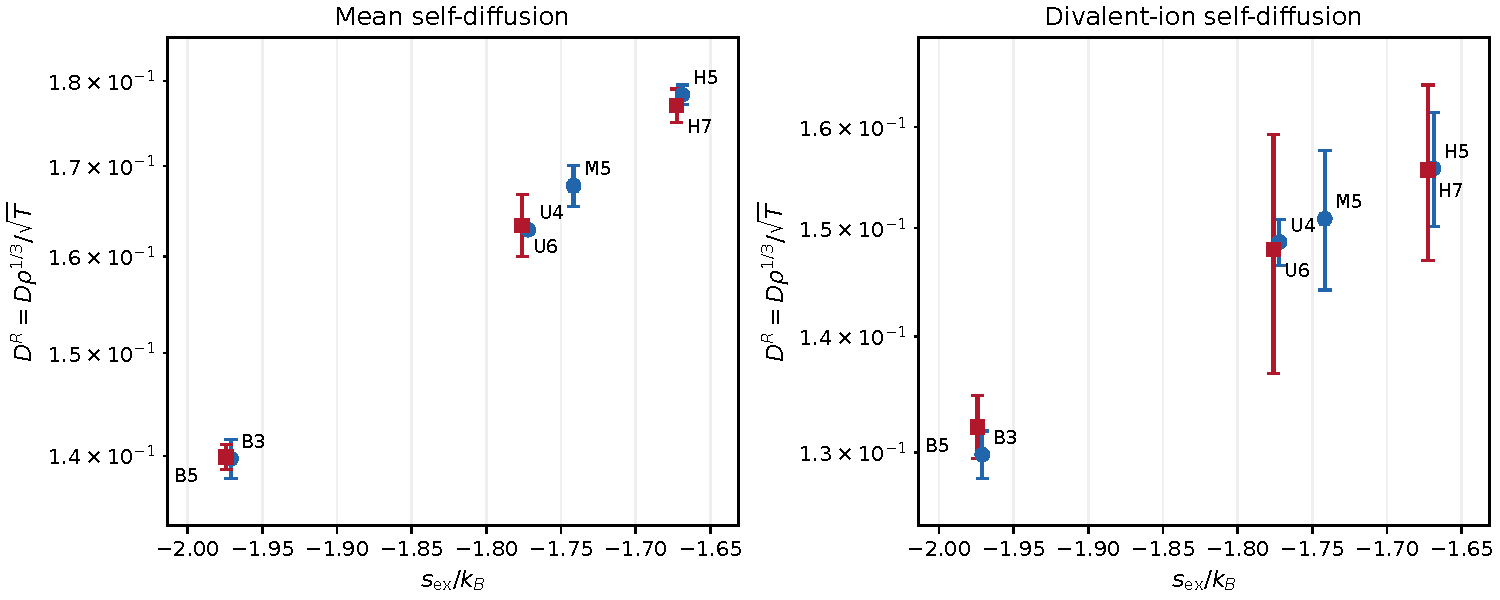
\includegraphics[width=\textwidth]{figures/component_entropy_diffusion.pdf}
\caption{Rosenfeld-reduced mean and divalent-probe self-diffusion versus replicated MD excess entropy. Vertical axes are logarithmic. Blue circles: no monovalent background; red squares: 5\% of each monovalent sign. Bars are nominal 95\% absolute-state replica intervals. L5 coincides exactly with U4 in transport and is omitted as a duplicate. The broad positive trend does not fix the slope of controlled composition changes.}
\label{fig:new_scaling}
\end{figure*}

The controlled local response differs from the broad-family fit. For H5/U4, $\Delta\ln D/\Delta(s_{\rm ex}/k_B)$ is approximately $0.88$ for the mean and $0.46$ for probes; H7/U6 gives approximately $0.78$ and $0.49$. The probe response is weaker than the mean response under the same intervention. Mean self-diffusion assigns only 6\% weight to divalent particles and cannot determine their mobility separately. The new results support a restricted entropy--mobility association for both observables, while neither component count nor a single bulk entropy establishes a universal species law. No association-lifetime mechanism has yet been measured in this study.

\subsection{Estimator Sensitivity and Charge-Sign Symmetry}

The controlled ion point estimates remain positive, approximately 4--6\%, across the MSD windows (Table~\ref{tab:new_windows} and Fig.~\ref{fig:new_windows}). However, H5/U4 loses nominal significance over 50--200$\tau$: $+3.94\%$, interval $[-8.44,18.00]\%$. H7/U6 is unresolved in all three windows. Accordingly the approximately 5\% ion effect is a provisional trend, not a converged precise enhancement. VACF integrals support the broad mobility ordering, but do not independently resolve such a small effect with the present final-$100\tau$ records.

% Generated by generate_component_study_assets.py; do not edit numbers by hand.
\begin{table*}[t]
\centering
\caption{Sensitivity of the paired divalent-ion diffusion change (percent) to MSD fitting window, with nominal 95\% replica intervals. The 20--100$\tau$ window is primary. The positive controlled effect is not uniformly significant across estimators/windows.}
\label{tab:new_windows}
\small
\resizebox{\ifdim\width>\textwidth\textwidth\else\width\fi}{!}{%
\begin{tabular}{lrrr}
\toprule
Comparison & 10--50$\tau$ & 20--100$\tau$ & 50--200$\tau$ \\
\midrule
H5/U4 & $+5.92\;[+1.87,+10.13]$ & $+4.81\;[+0.60,+9.19]$ & $+3.94\;[-8.44,+18.00]$ \\
H7/U6 & $+5.31\;[-1.17,+12.22]$ & $+5.20\;[-6.14,+17.92]$ & $+4.46\;[-5.66,+15.67]$ \\
\bottomrule
\end{tabular}}
\end{table*}


\begin{figure}[tb]
\centering
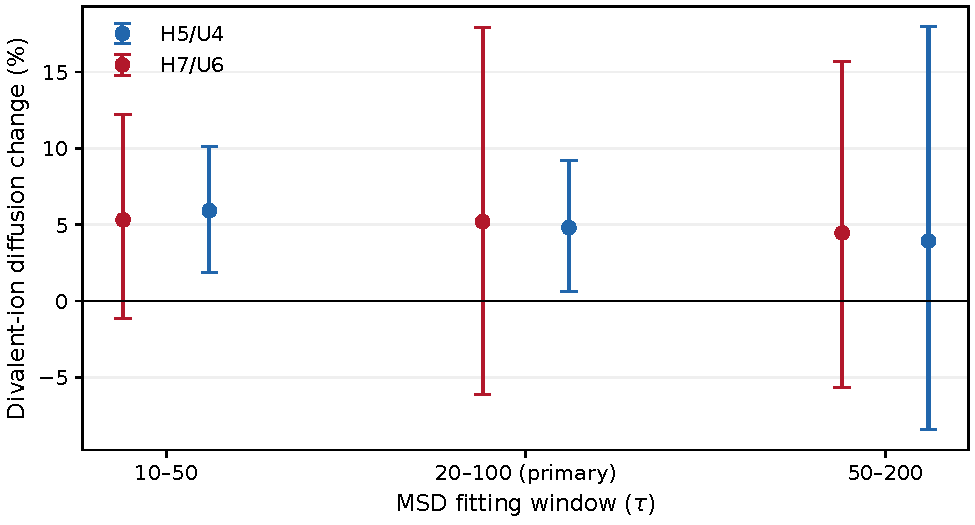
\includegraphics[width=\linewidth]{figures/component_window_sensitivity.pdf}
\caption{Controlled divalent-ion diffusion changes and nominal paired 95\% intervals for alternative MSD windows. The point estimates are consistently positive, but statistical significance is sensitive to the fitting window and monovalent background.}
\label{fig:new_windows}
\end{figure}

Charge-sign symmetry remains a convergence diagnostic. The B3 model is invariant under global charge reversal, yet its primary-window estimate gives $D_{+2}-D_{-2}=0.01039$, nominal replica interval $[0.00291,0.01786]$. The other states have sign-difference intervals containing zero. Generated inputs use identical masses and LJ parameters for both probe signs, random probe assignments, one all-particle thermostat, and a common COM frame; no sign-dependent input parameter was found. The B3 asymmetry nevertheless flags remaining sampling or uncertainty-estimation limitations. Pooling the signs does not remove that concern. It also does not explain away the large baseline contrasts, for which each sign separately increases.

Across all 24 replicas, switching from cubic to shape-preserving interpolation changes dense-state entropy by at most $0.00032k_B$. Retaining all or 75\% of production instead of the final half changes it by at most $0.00165k_B$. These sensitivities are small relative to the $0.103k_B$ diversification increments, but they do not bound finite-size bias or error below the lowest simulated density. Low-wavevector species concentration-fluctuation diagnostics remain of order unity, approximately 0.48--1.80 for individual replica/species values, with no large enhancement in the selected mixtures. One box size and these trajectory lengths cannot exclude slower segregation or establish phase stability.

% Shared rehabilitation results for the paper and technical report.
\subsection{Rehabilitation and Limits of the 2PT Excess Entropy}
\label{sec:2pt_rehabilitation}

We reanalyzed the existing final-$100\tau$ velocity records of all 24 replicas using a corrected classical two-phase thermodynamic (2PT) estimator. The revised spectral construction follows Sun \emph{et al.}~\cite{Sun2017}, with the equal-partial-volume mixture approximation discussed by Lai \emph{et al.}~\cite{Lai2012}. Each species is assigned $\bar V_i=1/\rho$; equal nominal diameters do not establish equality of actual partial volumes in these charged, dispersion-diverse liquids. The primary gas/solid partition exponent is $\delta=1$; the published LJ value $\delta=1.5$ is an unfitted sensitivity. Neither partition, reference volume, nor entropy offset is adjusted to match thermodynamic integration (TI).

The calculation corrects the density scaling and prefactor of the normalized diffusivity ($\Delta\propto D\sqrt{m/T}\rho^{1/3}$), weights gas entropy by its gas-like fraction, and subtracts the classical ideal-mixture reference consistently. The complete finite-record autocorrelation, in the common system-COM frame, is Gaussian-tapered with primary width $10\tau$. Its spectrum spans the full Nyquist band and is normalized by measured $C(0)$ to three modes per particle; raw target-temperature mode counts are retained as a diagnostic. The gas Lorentzian and its entropy tail are integrated analytically to infinity. The residual spectrum is kept signed as revised-2PT bookkeeping, rather than clipped to a positive ``solid population.'' This partition is not a literal count of free ions or bound oscillators.

Seven analytic checks pass, including the standard fluidicity polynomial, unit invariance, a solvable VACF/Green--Kubo limit, the Lorentzian entropy tail, the dilute-gas limit, and classical-reference and label/mixing cancellation. Normalization, reconstruction, and independence of the arbitrary classical phase-space constant hold to floating-point precision. Mechanically identical labels are pooled before the nonlinear entropy estimate. For all three actual U4/L5 pairs, matched retained particle IDs have identical COM-corrected velocity hashes, VACFs, and resulting 2PT entropies. Separately processing the label samples gives a difference $+0.00062k_B$, interval $[-0.00428,0.00553]k_B$, consistent with sampling. State-mean pooled-probe spectral diffusivities agree with the full-production MSD coefficients within $2.6\%$.

\begin{figure*}[t]
\centering
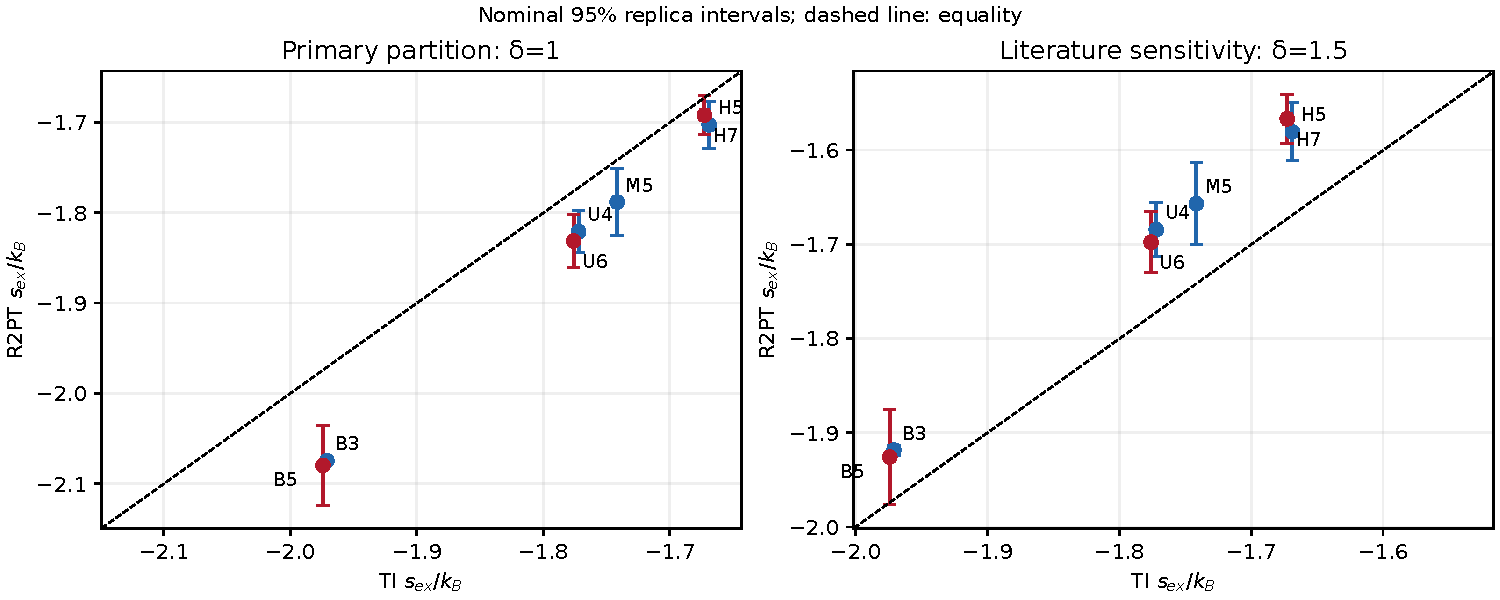
\includegraphics[width=\textwidth]{figures/component_2pt_validation.pdf}
\caption{Corrected classical revised-2PT excess entropy against TI for the seven mechanically distinct mixtures. L5 duplicates U4 in transport and is omitted. Bars are nominal 95\% absolute-state replica intervals; dashed lines denote equality. The left panel uses the primary partition $\delta=1$, and the right panel the unfitted literature sensitivity $\delta=1.5$. Internal consistency does not remove composition-dependent thermodynamic bias.}
\label{fig:2pt_validation}
\end{figure*}

These successes rehabilitate the implementation, but not its quantitative thermodynamic accuracy across compositions (Fig.~\ref{fig:2pt_validation}). For B3 the primary estimate is $-2.07445k_B$, compared with TI $-1.97101k_B$: the approximately $3.4k_B$ discrepancy of the archived $-5.376k_B$ result is reduced to $0.10344k_B$. Primary absolute biases range from about $-0.019$ to $-0.105k_B$, with all nominal paired bias intervals below zero. B3, B5, and U6 exceed the prespecified practical mean-bias tolerance $0.05k_B$. Thus the remaining error is composition dependent and comparable to the controlled entropy signal; a constant offset is insufficient.

% Generated by generate_component_study_assets.py; do not edit numbers by hand.
\begin{table*}[t]
\centering
\caption{Controlled excess-entropy increments from TI and corrected classical revised 2PT. All entropy quantities are per particle in $k_B$. Bias is the paired difference between the 2PT and TI increments; brackets are nominal 95\% Student-$t$ intervals from three independent replica pairs (two degrees of freedom), without multiplicity correction. The primary partition is $\delta=1$; $\delta=1.5$ is an unfitted sensitivity.}
\label{tab:2pt_contrasts}
\small
\resizebox{\ifdim\width>\textwidth\textwidth\else\width\fi}{!}{%
\begin{tabular}{llrrr}
\toprule
Comparison & Partition & TI $\Delta s_{\rm ex}/k_B$ & 2PT $\Delta s_{\rm ex}/k_B$ & Bias [95\% CI] \\
\midrule
H5/U4 & $\delta=1$ & 0.10322 & 0.11818 & $+0.01496\;[-0.00544,+0.03536]$ \\
H5/U4 & $\delta=1.5$ & 0.10322 & 0.10397 & $+0.00075\;[-0.02175,+0.02326]$ \\
H7/U6 & $\delta=1$ & 0.10331 & 0.13927 & $+0.03596\;[+0.01501,+0.05692]$ \\
H7/U6 & $\delta=1.5$ & 0.10331 & 0.13086 & $+0.02755\;[+0.00705,+0.04805]$ \\
\bottomrule
\end{tabular}}
\end{table*}


For H5/U4, primary 2PT gives $\Delta s_{\rm ex}=0.11818k_B$ versus TI $0.10322k_B$, a point bias $+0.01496k_B$ (Table~\ref{tab:2pt_contrasts}). This meets the practical point-bias tolerance $0.02k_B$ and is statistically consistent with zero bias, but the wide interval does not establish equivalence within that tolerance. For H7/U6, the estimate is $0.13927k_B$ versus $0.10331k_B$, an approximately $35\%$ overestimate; its bias interval $[0.01501,0.05692]k_B$ excludes zero. The $\delta=1.5$ partition improves the first increment to $0.10397k_B$ but still overestimates the second at $0.13086k_B$. Agreement for one pair does not validate a partition for all compositions.

The discrepancies survive sensitivity checks. State-mean entropy spans over taper widths 5, 10, and $20\tau$ are $0.011$--$0.022k_B$; first/last-half record shifts reach $0.012k_B$. Frequency-grid refinement changes means by less than $0.00002k_B$, and sampling-interval decimation changes them by at most $0.0022k_B$. Illustrative volume-conserving $\pm10\%$ partial-volume perturbations shift means by at most $0.0032k_B$, without establishing that the equal-volume approximation is exact. Positive-part clipping would add modes: the signed negative residual represents approximately 2.3--3.9\% of the total mode weight in primary species spectra. The corrected bookkeeping avoids this artifact, but cannot eliminate the model dependence of the gas/solid partition.

We therefore retain TI as the entropy coordinate in the Rosenfeld analysis. Corrected 2PT and the underlying VACFs remain useful dynamical diagnostics, but species spectral allocations are not independently measured partial molar entropies. Because diffusion enters the zero-frequency spectrum and fluidicity construction, a 2PT--diffusion correlation is not an independent confirmation of entropy-driven enhancement. Probe fluidicity rises from about 0.530 in B3 to 0.569 in H5, consistent with increased low-frequency motion. However, the mean probe VACFs remain positive over the first $\tau$; a pronounced early negative backscattering minimum is not supported. Association populations and residence times, rather than a literal interpretation of the 2PT partition, are needed to test local-caging mechanisms.


\subsection{Further Discriminating Checks}

The first priority is longer independent matched replicas of U4/H5 and U6/H7, together with extended B3 sampling to resolve the charge-sign flag. Next, repeat matched states with $N=8000$ or $16000$ at fixed density and composition. Box-size effects need not cancel between liquids with different viscosity. Particle-size variation is a separate perturbation of packing, contact electrostatic coupling, and friction and should not be conflated with this box-size test.

Existing trajectories permit probe--solvent and probe--ion RDFs, coordination populations, association lifetimes, and exchange-time analysis. Species-resolved pair entropy could help explain local mobility, but is not a thermodynamic partial molar entropy or a replacement for total excess entropy. These measurements would test local caging and association mechanisms without inferring kinetics from static entropy alone.

After convergence tests, increasing $x_{+2}=x_{-2}$ symmetrically, for example to 0.06 or 0.10, would strengthen the ionic contribution and alter screening and association. Uniform/diverse solvents should be compared at matched concentration and ionic strength within each pair, with HNC re-screening and homogeneity checks. Several densities and temperatures at fixed composition, and states with matched excess entropy but different compositions, would distinguish state-point scaling from composition-induced correlations.
